\documentclass[]{plan}
\usepackage{graphicx}
\usepackage{hyperref}


%%%%%%%%%%%%%%%%%%%%%%
%%% Project Details
\def\studentname{Eman Naveed}
\def\reportyear{2024}
\def\projecttitle{Lindenmayer Systems}
\def\supervisorname{Anand Subramoney}
\def\degree{BSc (Hons) in Computer Science}
\def\fullOrHalfUnit{Full Unit} 

\begin{document}

\maketitle

%%%%%%%%%%%%%%%%%%%%%%
%%% ABSTRACT

\begin{abstract}
Lindenmayer systems(L-systems) were conceived as a mathematical theory of plant development. Prior to Aristid Lindenmayer's introduction of L-systems, an idea was brought up to use character strings to describe images. The concept being that objects could be recognized by coding their images and analyzing the resulting strings. The conclusion of conducted studies proved, however, that languages corresponding to intuitively simple classes of images - even those as simple as rectangles in a square grid - were all context-sensitive, while most practically useful results of formal language theory referred to context-free languages~\cite{HAN:1989}.

The basic L-system uses \textit{rewriting rules} or \textit{productions} to generate a complex object by recursively replacing parts of an initial much simpler object~\cite{PRU:1990}. A common example of the phenomenon is the Koch snowflake that shows the rewriting rules most clearly. Mandelbrot, in his description of this phenomenon, uses the terms \textit{initiator} and \textit{generator} to distinguish the initial simple shape and the line that replaces parts of the shape at each step of recursion. 
\begin{figure}[h]
\centering
%\fboxsep 2mm
\framebox{
	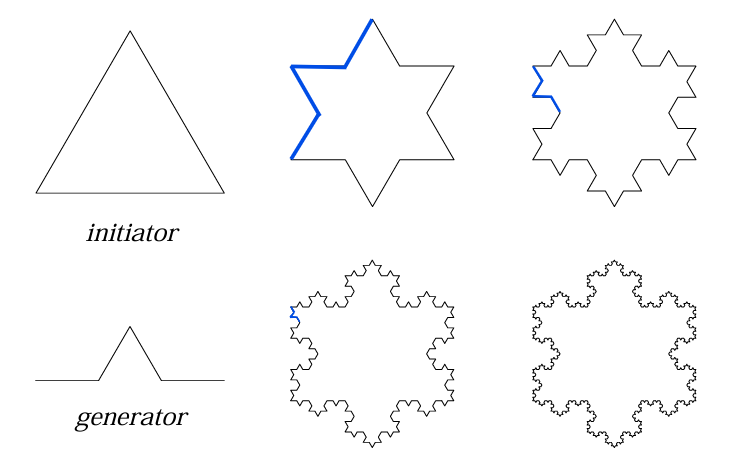
\includegraphics[width=12cm]{koch_curve} 
}
\caption{\label{fig:koch_curve} Construction of the Koch snowflake curve.}
\end{figure}

The distinction provided by L-systems from Chomsky grammars lay in the method of applying productions. While in Chomsky grammars, production are applied sequentially, one at a time, L-systems apply them in parallel so all letters in a given word are replaced simultaneously.

L-systems were introduced specifically to model plant development and so initial research and implementation of their functionalities circled around understanding and simulating organic structures. Experimentation with graphics continued to advance until Alvy Ray Smith demonstrated the use of L-systems for realistic image synthesis~\cite{SMT:1984}. There also exist applications of L-systems in the context of medicine, architecture, and music that are used for study and further research into the respective fields. 

Specifically, in the context of coding these systems, we will associate specific characters or letters to corresponding graphical representation - which in 2D Turtle graphics may simply be lines of arbitrary length or turns of arbitrary angle~\cite{MCL:2005}. These graphics of the fractals themselves will be defined entirely by strings of those characters or letters and all production will also be generated through those strings. The graphical output will show the image at each stage of rendering as the shape gets more and more complex. To ensure all these progressions remain visible in the window, the generator will reduce in size and be displaced in such a way that the overall graphic remains in its relative position and as its relative size(as shown in Figure 1 previously).

The project's specific requirements expect an initial implementation of non-stochastic L-systems - lacking the randomness incorporated into the rewriting rules of stochastic L-systems which allow for multiple possible outcomes from any given string - which should later be extended to support stochastic productions and mimic plant growth. 

My basic plan for the GUI layout is to have options to select some presets of specific fractals that would show the progression of iterations of each production. Alongside these would be the option to create a user's own fractal by allowing the selection of number of sides of the initiator and then the amount and complexity of generators that would dictate the rewriting rules. The iterations for this kind of functionality will have to be experimented with so the final product does not lag during rendering.

As this will be my first time building a UI of this complexity from scratch, I have only considered a few libraries to work with, though I require more research to understand them. My main choices of libraries to use are Java Swing or Processing which I will be able to decide between once I delve into coding.

I hope to experiment with different existing productions and attempt my own. A curiosity I'd like to explore is the Mandelbrot Set and whether I could reproduce a similar graphic through my own understandings of the system I will be attempting to build. This aspect would likely fall under non-stochastic implementation as it is an already mathematically defined motif. I plan to attempt reconstruction of specific plant structures in my stochastic implementations in an effort to mimic leaves and petals individually, although the assumption would be that a singular petal may be depicted as a generator instead of a final image. Also, I wish to explore 3D depiction of organic(possibly protein synthesis or simple fossils such as ammonite) and inorganic(Michael Hansmeyer's architectural forms~\cite{HANS:2003}) structures, though I will not be adding this to my initial timeline.

\end{abstract}
\newpage

{\textsf{\textbf{\LARGE{Timeline}}}}

Ideally, I hope to stick to this timeline as closely as possible. I hope to have all early deliverables and some aspects of final deliverables functional by end of Term 1 in December. Term 2 will have most of the GUI implementation so I have sufficient time to resolve any issues that may come with using software or libraries I am unfamiliar with. 

I plan to carry out testing throughout so I have not mentioned it explicitly except for after final functionality is achieved. The 3D implementation will likely be preset graphics unless I finish with the rest of the project earlier than expected as adding user interaction to 3D modeling may raise too many issues to resolve within the timeframe. 
\newline
\newline

\textbf{\Large{Term 1}}
\renewcommand{\arraystretch}{1.5}
    
\begin{tabular}{c|p{12cm}}
    Week beginning\\
    \hline
    
    21st October & Begin on simple non-stochastic implementation and report draft. Have worked examples for the report completed by end of week.\\
    28th October & Begin research of graphics libraries and be ready to start implementation by end of week. Have coding for at least three simple fractals completed and ready to render\\
    4th November & Begin graphics rendering and add more complex fractals(Mandelbrot Set or Julia Set; consider Lyapunov fractal). Add findings and progress to report draft\\
    11th November & Have graphics rendering at least semi-functional, continue to refine code as necessary to get accurate and expected results. Rendering capabilities must be fully functional by end of week. Review progress with Anand\\
    18th November & Research further classes of L-systems and add findings to report\\
    25th November & Research stochastic implementation and begin coding for it. Have at least 2 examples ready for rendering by end of week. Begin adding variable parameters if finished with stochastic implementation before time\\
    2nd December & Add all progress and findings to report draft. Review overall progress with Anand. Begin work on presentation. Have first draft compiled, and ready to review and edit by end of week\\
    9th December & Continue work on interim report, review when necessary. Complete presentation\\
\end{tabular}
\newpage

\textbf{\Large{Term 2}}
\renewcommand{\arraystretch}{1.5}

\begin{tabular}{c|p{12cm}}
    Week beginning\\
    \hline

    20th January & Add functionality for user-given parameters. Have functional with rendering by end of week\\
    27th January & Research and begin implementing GUI beyond simple rendering. Have semi-functional GUI by end of week\\
    3rd February & Begin compiling final report draft and continue work on GUI\\
    10th February & Have GUI fully functional and begin research on L-system plant mimics. Review progress with Anand\\
    17th February & Begin work on plant mimics and have functional for rendering by end of week\\
    24th February & Take the week to review and work on report draft. Have users experiment with the UI and alter functionality where necessary\\
    3rd March & Research 3D implementation and software or libraries needed for it if existing system cannot manage\\
    10th March & Begin 3D implementation and update report draft with findings\\
    17th March & Have functional 3D implementation by end of week.\\
    24th March & Complete draft of final report and review with Anand.\\
    31st March & Complete final report and submit\\
\end{tabular}

\newpage

{\textsf{\textbf{\LARGE{Risks and Mitigations}}}}

\begin{enumerate}
    \item \textsf{\textbf{\large{Poor Time Management}}}
    
    Managing time effectively is vital for a project's completion within the set timeframe, otherwise tasks may overrun, stalling overall progress. In regards to my project, I will endeavour to divide time according to the complexity of the work required. Though I am likely to only get a better idea once I begin working, I have allowed sufficient leeway within my estimated timeline in order to avoid such issues.
    
    \item \textsf{\textbf{\large{Hardware Failure}}}
    
    It is possible that the machine in use for the execution of this project fails. There can be storage issues that could potentially cause loss in data and progress. I will remain diligent in keeping my repository up to date so there is no significant progress left out and risked during implementation.
    
    \item \textsf{\textbf{\large{Technical Challenges}}}
    
    Encountering unfamiliar technologies can stall progress, especially in a project such as this where I will be making of use of applications that I am unfamiliar with. I have made an effort to include sufficient research time into the timeline so that I can be efficient in my work when the time comes to begin use of such applications or framework.
    
    \item \textsf{\textbf{\large{Quality of Code}}}

    It is possible to overlook issues in the code when working individually that may be apparent when working with a team. I will be testing the code regularly and will endeavour to review progress with my supervisor when necessary. I will make use of the resources available when best applicable while making sure not to accidentally copy the exact demonstrations.

    \item \textsf{\textbf{\large{Hardware Limitations}}}

    As we progress through recursions in L-systems the complexity of the strings and their related graphics increases, hence requiring significant computational resources. This has the potential of creating performance issues that may stall code execution. I will test the software I use to ensure I know the limit of recursion depth that my machine can handle.

    \item \textsf{\textbf{\large{Rendering Quality}}} 

    L-systems work by scaling the productions in such a way that the generator is reduced in size and displaced so the overall figure remains in the window. After a number of iterations, the changes to the graphics this produces may become imperceptible. I will make sure to limit iteration to the point where changes can still be seen without requiring higher resolution than the default of most machines. 
    
    \item \textsf{\textbf{\large{Feasibility}}}

    When exploring new avenues and experimenting with complex implementation, it is easy to get carried away and lose track of time and programming capability. In case I am unable to achieve my particular goals within the time frame assigned for it, I will still have proof of base functionality and simpler examples for demonstration. Further trials can be postponed until after the specified requirements are completed.
    
    \item \textsf{\textbf{\large{Parametric Interaction}}}

    Allowing users to manipulate and build their own models - fractals or otherwise - can increase complexity greatly. It is important to develop an adaptive algorithm that can limit the number of iterations rendered according to the complexity of the fractal being generated.
    
\end{enumerate}



%%%% BIBLIOGRAPHY
\newpage
\begin{thebibliography}{99}
\addcontentsline{toc}{chapter}{Bibliography}
\bibitem{PRU:1990} Przemyslaw Prusinkiewicz and Aristid Lindenmayer. \emph{The Algorithmic Beauty of Plants}.  Springer-Verlag, New York, 1990.
\bibitem{HAN:1989} Przemyslaw Prusinkiewicz and James Hanan. \emph{Lindenmayer systems, fractals, and plants}. Springer-Verlag, Berlin, 1989.
\bibitem{MCL:2005} Mark McClure. \emph{Parametric L-Systems and Borderline Fractals}. \emph{Mathematica in Education and Research}, 2005 
\bibitem{SMT:1984} Alvy Ray Smith. \emph{Plants, Fractals, and Formal Languages}. Lucasfilm, 1984.
\bibitem{HANS:2003} Michael Hansmeyer. \emph{L-Systems in Architecture}. 2003.
\end{thebibliography}
\label{endpage}



\end{document}
